\section{Mô hình Khuếch tán (Diffusion Models)}
\label{sec:diffusion_models}

Trong khi GANs thống trị lĩnh vực sinh ảnh trong nhiều năm, chúng vẫn tồn tại những thách thức cố hữu về sự ổn định trong huấn luyện và hiện tượng sụp đổ mode. Vào khoảng năm 2020, một họ mô hình sinh mới, lấy cảm hứng từ nhiệt động lực học, đã nổi lên và nhanh chóng chiếm lĩnh vị trí dẫn đầu: \textbf{Mô hình Khuếch tán (Diffusion Models)}. Với khả năng tạo ra những hình ảnh có chất lượng và sự đa dạng vượt trội, cùng với quá trình huấn luyện ổn định hơn, các mô hình khuếch tán đã mở ra một cuộc cách mạng sáng tạo mới, đặc biệt trong lĩnh vực tạo ảnh từ văn bản.

\subsection{Lý thuyết Cơ bản: Quá trình Khuếch tán và Khử nhiễu}
\label{subsec:diffusion_theory}

\textbf{Trực giác: Mực trong nước.}
Hãy tưởng tượng bạn nhỏ một giọt mực vào cốc nước trong. Ban đầu giọt mực có hình dạng rõ ràng. Sau vài giây nó lan ra. Sau vài phút nó hòa tan hoàn toàn --- cốc nước trở thành màu đồng nhất, không còn dấu vết gì của giọt mực ban đầu. Quá trình này là \textit{khuếch tán (diffusion)}: từ trật tự đến hỗn loạn.

Diffusion Models khai thác ý tưởng này theo chiều ngược: \textit{nếu ta có thể dạy máy tính học cách đảo ngược quá trình hỗn loạn --- từ nhiễu trở về ảnh --- thì ta có thể sinh ra ảnh mới bằng cách bắt đầu từ nhiễu ngẫu nhiên thuần túy.}

Hai quá trình cốt lõi:
\begin{enumerate}
    \item \textbf{Forward process} (quá trình thuận): Lấy ảnh sạch, từ từ thêm nhiễu qua $T$ bước ($T = 1000$ trong DDPM), cho đến khi ảnh biến thành nhiễu Gaussian thuần túy. Quá trình này \textit{cố định, không cần học}.
    \item \textbf{Reverse process} (quá trình ngược): Huấn luyện mạng nơ-ron học cách \textit{đảo ngược} --- nhận ảnh nhiễu và tìm ra ảnh ít nhiễu hơn một bước. Lặp lại $T$ bước từ nhiễu thuần túy để ra ảnh.
\end{enumerate}

\begin{center}
    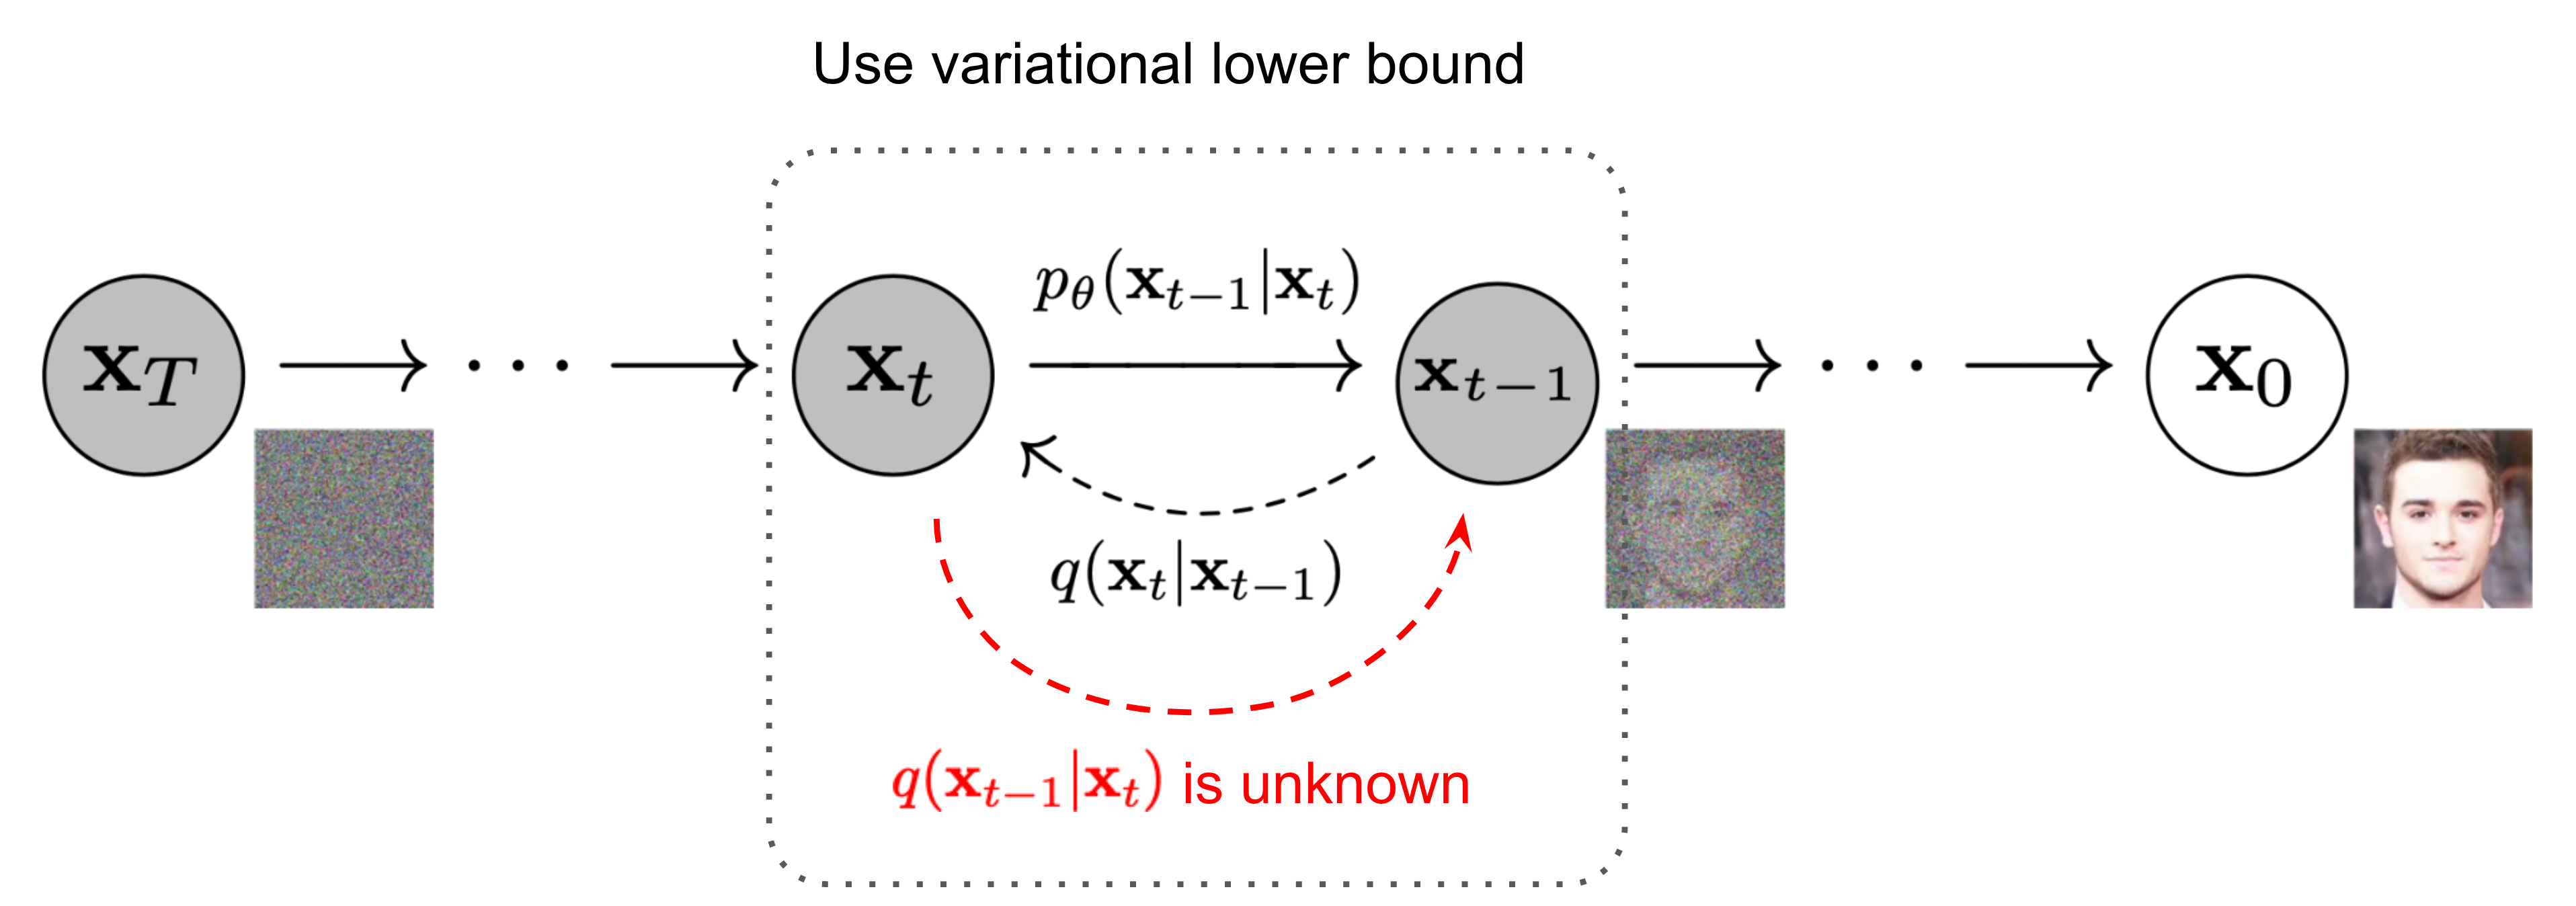
\includegraphics[width=0.98\textwidth]{images/ddpm_diffusion_process.png}
    \captionof{figure}{Hai quá trình của Diffusion Model: forward process (trái sang phải) thêm nhiễu dần dần qua $T$ bước, reverse process (phải sang trái) dùng U-Net khử nhiễu từng bước trở về ảnh gốc.}
    \label{fig:diffusion_two_process}
\end{center}

\subsubsection{DDPM (Denoising Diffusion Probabilistic Models)}
\label{subsubsec:ddpm}

\textbf{DDPM} \cite{Ho2020} (Ho et al., 2020) là công trình đặt nền móng cho mọi diffusion model hiện đại. Trước khi vào công thức, hãy làm quen với ký hiệu.

\begin{mdframed}[style=infobox]
\textbf{Bảng ký hiệu toán học --- Đọc phần này trước}

\begin{itemize}
    \item $\mathbf{x}_0$ --- ảnh gốc sạch (subscript 0 = bước 0, chưa có nhiễu). \textbf{x} in đậm vì đây là vector/ma trận (toàn bộ pixel của ảnh), không phải số vô hướng.
    \item $\mathbf{x}_t$ --- ảnh sau khi thêm nhiễu qua $t$ bước ($t = 1, 2, \ldots, T$).
    \item $\mathcal{N}(\mu, \sigma^2)$ --- \textbf{phân phối Gaussian} (phân phối chuẩn) với giá trị trung bình $\mu$ và phương sai $\sigma^2$. Khi ta lấy mẫu $x \sim \mathcal{N}(\mu, \sigma^2)$, ta lấy ngẫu nhiên một số thực quanh $\mu$, độ tản mát được xác định bởi $\sigma^2$.
    \item $\mathcal{N}(\mathbf{0}, \mathbf{I})$ --- Gaussian chuẩn: trung bình bằng 0, phương sai bằng 1 ở mỗi chiều. $\mathbf{I}$ là ma trận đơn vị (identity matrix), tức là các chiều độc lập nhau.
    \item $\boldsymbol{\epsilon} \sim \mathcal{N}(\mathbf{0}, \mathbf{I})$ --- lấy mẫu vector nhiễu ngẫu nhiên từ Gaussian chuẩn. $\boldsymbol{\epsilon}$ có cùng kích thước với ảnh (mỗi pixel nhận một giá trị nhiễu).
    \item $\beta_t \in (0, 1)$ --- lượng nhiễu thêm vào ở bước $t$. Giá trị nhỏ (0.0001 đến 0.02).
    \item $\alpha_t = 1 - \beta_t$ --- tỷ lệ tín hiệu ảnh gốc còn lại sau bước $t$ (gần 1).
    \item $\bar{\alpha}_t = \alpha_1 \cdot \alpha_2 \cdots \alpha_t$ --- tích tích lũy, tỷ lệ tín hiệu gốc còn lại sau \textit{tất cả} $t$ bước.
    \item $\mathbb{E}[\cdot]$ --- giá trị kỳ vọng (trung bình). $\mathbb{E}_{t, \mathbf{x}_0, \boldsymbol{\epsilon}}[\ldots]$ nghĩa là lấy trung bình trên: các bước $t$ ngẫu nhiên, ảnh gốc $\mathbf{x}_0$ trong dataset, và nhiễu $\boldsymbol{\epsilon}$ ngẫu nhiên.
    \item $\theta$ (theta) --- tham số của mạng nơ-ron (trọng số cần học).
    \item $\boldsymbol{\epsilon}_\theta(\mathbf{x}_t, t)$ --- mạng nơ-ron tham số hóa bởi $\theta$, nhận đầu vào là ảnh nhiễu $\mathbf{x}_t$ và bước thời gian $t$, dự đoán nhiễu.
\end{itemize}
\end{mdframed}

\paragraph{Quá trình Thuận (Forward Process) --- Phá hủy ảnh có kiểm soát.}

Bắt đầu từ ảnh sạch $\mathbf{x}_0$, ở mỗi bước $t$ ta thêm một lượng nhỏ nhiễu Gaussian:

\begin{equation}
    q(\mathbf{x}_t \mid \mathbf{x}_{t-1}) = \mathcal{N}\!\left(\mathbf{x}_t;\; \underbrace{\sqrt{1-\beta_t}}_{\text{co lại tín hiệu}}\,\mathbf{x}_{t-1},\;\; \underbrace{\beta_t\,\mathbf{I}}_{\text{thêm nhiễu}}\right)
\end{equation}

\textbf{Đọc công thức này như sau:} ``Ảnh ở bước $t$ bằng ảnh bước trước nhân với $\sqrt{1-\beta_t}$ (co nhẹ lại để giữ tổng phương sai ổn định), cộng thêm nhiễu ngẫu nhiên có phương sai $\beta_t$.'' Lý do nhân $\sqrt{1-\beta_t}$ chứ không phải $(1-\beta_t)$: phương sai của tổng hai biến độc lập bằng tổng phương sai --- cần nhân với căn để không tích lũy nhiễu quá nhanh (đây là chi tiết kỹ thuật để giữ variance scheduling hợp lý).


\textbf{Trick quan trọng: Nhảy thẳng đến bước $t$ bất kỳ.}

Nếu cần chạy 1000 bước tuần tự mỗi lần, training sẽ cực chậm. May mắn là từ tính chất của Gaussian, ta có thể tính \textit{trực tiếp} $\mathbf{x}_t$ từ $\mathbf{x}_0$ mà không cần đi qua $t-1$ bước trung gian:

\begin{equation}
    \mathbf{x}_t = \underbrace{\sqrt{\bar{\alpha}_t}}_{\text{tỷ lệ ảnh gốc}} \cdot \mathbf{x}_0 \;+\; \underbrace{\sqrt{1 - \bar{\alpha}_t}}_{\text{tỷ lệ nhiễu}} \cdot \boldsymbol{\epsilon}, \qquad \boldsymbol{\epsilon} \sim \mathcal{N}(\mathbf{0}, \mathbf{I})
    \label{eq:ddpm_forward_direct}
\end{equation}

\textbf{Đọc công thức này như sau:} ``Ảnh nhiễu ở bước $t$ bằng ảnh gốc nhân $\sqrt{\bar{\alpha}_t}$ cộng với nhiễu thuần túy nhân $\sqrt{1 - \bar{\alpha}_t}$.'' Khi $t$ nhỏ (đầu quá trình): $\bar{\alpha}_t \approx 1$, tức $\mathbf{x}_t \approx \mathbf{x}_0$ (ảnh gần như nguyên). Khi $t = T$ (cuối): $\bar{\alpha}_T \approx 0$, tức $\mathbf{x}_T \approx \boldsymbol{\epsilon}$ (nhiễu thuần túy). Công thức này là \textbf{reparameterization trick} --- giúp training chọn bước $t$ ngẫu nhiên bất kỳ và tạo ngay $\mathbf{x}_t$ mà không cần vòng lặp.


\paragraph{Quá trình Ngược (Reverse Process) --- Tại sao cần mạng nơ-ron?}

Nếu forward process là $q(\mathbf{x}_t \mid \mathbf{x}_{t-1})$, ta muốn biết chiều ngược: $q(\mathbf{x}_{t-1} \mid \mathbf{x}_t)$ --- ``biết ảnh nhiễu $\mathbf{x}_t$, ảnh ít nhiễu hơn $\mathbf{x}_{t-1}$ là gì?''

Vấn đề: để tính chính xác $q(\mathbf{x}_{t-1} \mid \mathbf{x}_t)$, cần biết toàn bộ phân phối dữ liệu thật $p(\mathbf{x}_0)$ --- chính là thứ ta đang cố học. Đây là bài toán gà-trứng.

Giải pháp: dùng mạng nơ-ron $p_\theta(\mathbf{x}_{t-1} \mid \mathbf{x}_t)$ để \textit{xấp xỉ} phân phối ngược này. Mạng học từ dữ liệu huấn luyện để biết: ``từ ảnh nhiễu ở bước $t$, một bước khử nhiễu hợp lý dẫn đến đâu?''

\textbf{Mạng nơ-ron học gì?} Thay vì dự đoán trực tiếp $\mathbf{x}_{t-1}$ (một ảnh hoàn chỉnh, khó học), DDPM dạy mạng học cách \textbf{dự đoán nhiễu $\boldsymbol{\epsilon}$} đã được thêm vào ở bước $t$. Từ nhiễu dự đoán, ta tính ngược lại được $\mathbf{x}_{t-1}$.

Tại sao dự đoán nhiễu dễ hơn? Vì nhiễu $\boldsymbol{\epsilon}$ là Gaussian chuẩn --- một phân phối đơn giản, rõ ràng, không phụ thuộc nội dung ảnh. Dự đoán ``cái gì đã được thêm vào'' dễ hơn dự đoán ``ảnh ban đầu trông như thế nào.''

\begin{center}
    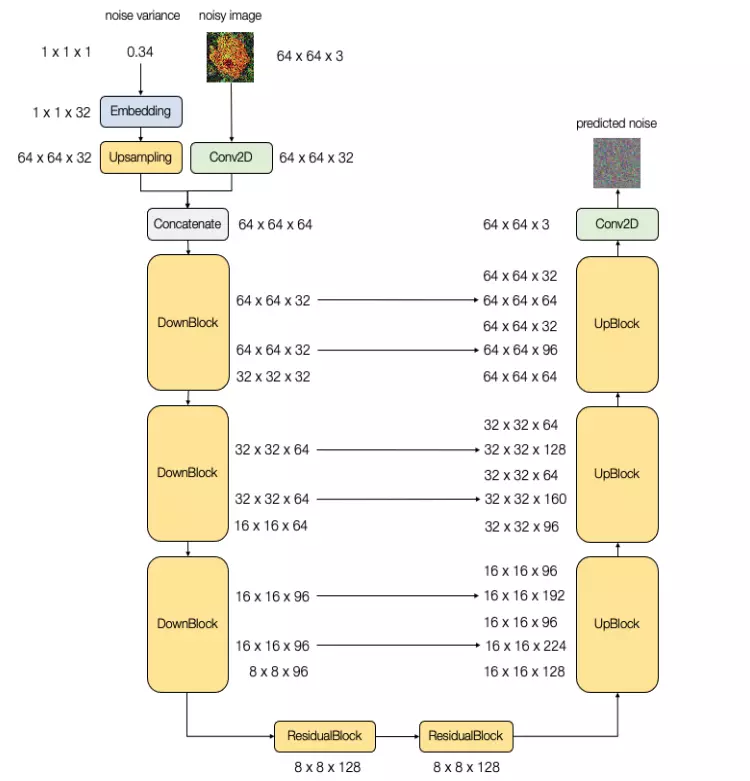
\includegraphics[width=0.85\textwidth]{images/diffusion_c890b55f.png}
    \captionof{figure}{Kiến trúc U-Net trong DDPM: ảnh nhiễu $\mathbf{x}_t$ ($64\times64\times3$) và noise variance được embed thành vector $1\times1\times32$ rồi upsample. Các DownBlock giảm dần độ phân giải, UpBlock khôi phục với skip connections. Đầu ra là ảnh nhiễu dự đoán $\hat{\boldsymbol{\epsilon}}$ cùng kích thước đầu vào.}
    \label{fig:unet_ddpm}
\end{center}

\textbf{Kiến trúc U-Net và Time Embedding.}
Mạng nơ-ron $\boldsymbol{\epsilon}_\theta(\mathbf{x}_t, t)$ cần nhận \textit{hai} đầu vào: ảnh nhiễu $\mathbf{x}_t$ và bước thời gian $t$. U-Net xử lý $\mathbf{x}_t$ qua các lớp encoder/decoder với skip connections. Bước thời gian $t$ được chuyển thành một vector embedding bằng \textbf{sinusoidal positional encoding} (tương tự Transformer) rồi cộng vào mỗi lớp của U-Net. Nhờ đó, cùng một mạng xử lý đúng cách cho từng mức độ nhiễu khác nhau --- bước $t = 100$ (ảnh hơi mờ) và bước $t = 900$ (gần như nhiễu) cần xử lý rất khác nhau.

\begin{center}
    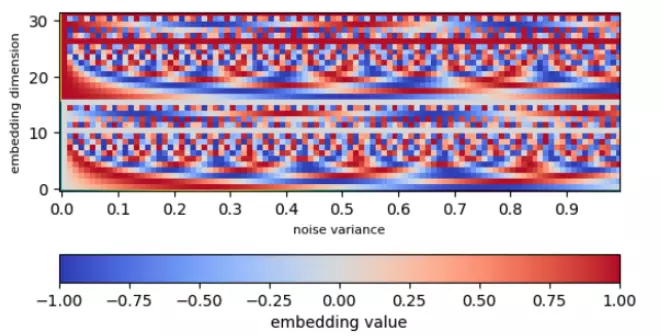
\includegraphics[width=0.85\textwidth]{images/diffusion_8c11024e.png}
    \captionof{figure}{Trực quan hóa sinusoidal time embedding: trục ngang là giá trị noise variance (tương ứng bước $t$), trục dọc là các chiều của embedding vector. Mỗi bước $t$ tạo ra một ``chữ ký'' embedding riêng biệt, giúp U-Net phân biệt được mình đang khử nhiễu ở giai đoạn nào.}
    \label{fig:time_embedding}
\end{center}

\paragraph{Hàm mất mát --- Đơn giản đến bất ngờ.}

Sau khi qua nhiều phép toán xác suất (ELBO, KL divergence), hàm mất mát của DDPM được đơn giản hóa thành:

\begin{equation}
    \mathcal{L}_{\text{simple}} = \mathbb{E}_{t \sim [1,T],\; \mathbf{x}_0 \sim \text{data},\; \boldsymbol{\epsilon} \sim \mathcal{N}(\mathbf{0},\mathbf{I})}
    \Bigl[\;
    \underbrace{\bigl\|\boldsymbol{\epsilon} - \boldsymbol{\epsilon}_\theta(\underbrace{\sqrt{\bar{\alpha}_t}\,\mathbf{x}_0 + \sqrt{1-\bar{\alpha}_t}\,\boldsymbol{\epsilon}}_{\mathbf{x}_t \text{ theo công thức (\ref{eq:ddpm_forward_direct})}},\; t)\bigr\|^2}_{\text{MSE giữa nhiễu thật và nhiễu dự đoán}}
    \;\Bigr]
\end{equation}

\textbf{Đọc công thức này từng phần:}
\begin{itemize}
    \item $\mathbb{E}[\ldots]$: trung bình trên ngẫu nhiên --- chọn ngẫu nhiên một ảnh trong dataset, một bước $t$ ngẫu nhiên trong $[1, T]$, và một vector nhiễu $\boldsymbol{\epsilon}$ ngẫu nhiên.
    \item $\sqrt{\bar{\alpha}_t}\,\mathbf{x}_0 + \sqrt{1-\bar{\alpha}_t}\,\boldsymbol{\epsilon}$: đây chính là $\mathbf{x}_t$ --- ảnh nhiễu tại bước $t$ tính bằng reparameterization trick.
    \item $\boldsymbol{\epsilon}_\theta(\mathbf{x}_t, t)$: mạng nơ-ron dự đoán nhiễu từ $\mathbf{x}_t$ và $t$.
    \item $\|\boldsymbol{\epsilon} - \boldsymbol{\epsilon}_\theta(\cdots)\|^2$: MSE --- bình phương khoảng cách giữa nhiễu thật $\boldsymbol{\epsilon}$ và nhiễu dự đoán.
\end{itemize}

Nói ngắn gọn: \textit{thêm nhiễu ngẫu nhiên vào ảnh, cho mạng đoán nhiễu đó là gì, phạt nếu đoán sai.} Đơn giản như bài toán supervised learning thông thường.

\paragraph{Vòng lặp huấn luyện một bước.}

\begin{enumerate}
    \item Lấy một ảnh sạch $\mathbf{x}_0$ từ dataset.
    \item Chọn bước ngẫu nhiên $t \sim \text{Uniform}(1, T)$.
    \item Sinh nhiễu ngẫu nhiên $\boldsymbol{\epsilon} \sim \mathcal{N}(\mathbf{0}, \mathbf{I})$.
    \item Tính $\mathbf{x}_t = \sqrt{\bar{\alpha}_t}\,\mathbf{x}_0 + \sqrt{1-\bar{\alpha}_t}\,\boldsymbol{\epsilon}$ \hfill (không cần vòng lặp 1000 bước).
    \item Cho mạng dự đoán: $\hat{\boldsymbol{\epsilon}} = \boldsymbol{\epsilon}_\theta(\mathbf{x}_t, t)$.
    \item Tính loss: $\mathcal{L} = \|\boldsymbol{\epsilon} - \hat{\boldsymbol{\epsilon}}\|^2$.
    \item Backpropagation, cập nhật $\theta$.
\end{enumerate}


\paragraph{Quá trình Lấy mẫu --- Sinh ảnh mới.}

Sau khi huấn luyện xong, để sinh một ảnh hoàn toàn mới:

\begin{enumerate}
    \item Khởi đầu với nhiễu thuần túy: $\mathbf{x}_T \sim \mathcal{N}(\mathbf{0}, \mathbf{I})$ --- một ma trận pixel ngẫu nhiên, trông như tuyết trên TV.
    \item Lặp từ $t = T$ xuống $t = 1$: Dùng mạng để ước tính nhiễu: $\hat{\boldsymbol{\epsilon}} = \boldsymbol{\epsilon}_\theta(\mathbf{x}_t, t)$. Trừ bớt nhiễu để có $\mathbf{x}_{t-1}$:
    \[
        \mathbf{x}_{t-1} = \frac{1}{\sqrt{\alpha_t}}\!\left(\mathbf{x}_t - \frac{1-\alpha_t}{\sqrt{1-\bar{\alpha}_t}}\,\hat{\boldsymbol{\epsilon}}\right) + \underbrace{\sqrt{\beta_t}\,\mathbf{z}}_{\text{nhiễu nhỏ thêm vào}}, \quad \mathbf{z} \sim \mathcal{N}(\mathbf{0},\mathbf{I})
    \]
    \textbf{Tại sao lại cộng thêm nhiễu $\sqrt{\beta_t}\,\mathbf{z}$?} Đây là bước quan trọng: thêm một chút nhiễu ngẫu nhiên vào mỗi bước reverse giúp quá trình lấy mẫu có tính ngẫu nhiên --- mỗi lần chạy từ cùng $\mathbf{x}_T$ sẽ ra ảnh khác nhau, tránh mô hình chỉ sinh một ảnh duy nhất.
    \item Sau $T$ bước: $\mathbf{x}_0$ là ảnh mới được sinh ra.
\end{enumerate}

\begin{center}
    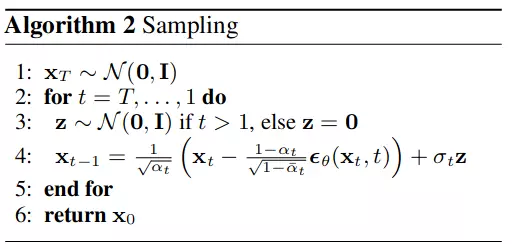
\includegraphics[width=0.65\textwidth]{images/diffusion_868fa263.png}
    \captionof{figure}{Thuật toán Sampling của DDPM (Algorithm 2): bắt đầu với $\mathbf{x}_T \sim \mathcal{N}(\mathbf{0},\mathbf{I})$, lặp $t$ từ $T$ về $1$ dùng mạng $\boldsymbol{\epsilon}_\theta$ để tính $\mathbf{x}_{t-1}$, trả về $\mathbf{x}_0$ là ảnh sinh ra.}
    \label{fig:ddpm_sampling}
\end{center}

\begin{mdframed}[style=infobox]
\textbf{DDPM là mô hình sinh ảnh \textit{không có điều hướng}}

DDPM thuần túy chỉ học phân phối của tập dữ liệu huấn luyện và sinh ảnh \textbf{ngẫu nhiên} từ đó. Nếu train trên ảnh khuôn mặt người, mỗi lần sample sẽ ra một khuôn mặt ngẫu nhiên --- bạn \textit{không thể} yêu cầu ``sinh khuôn mặt phụ nữ tóc dài'' hay ``sinh theo phong cách Van Gogh''. Không có cơ chế nào để người dùng can thiệp vào quá trình sinh.

Đây là giới hạn cốt lõi của DDPM gốc, và cũng là lý do cộng đồng nghiên cứu nhanh chóng phát triển các kỹ thuật \textit{conditional generation} để biến diffusion models từ công cụ ``sinh ngẫu nhiên'' thành công cụ ``sinh theo yêu cầu''.

\medskip
\textbf{Ưu điểm so với GAN:}
\begin{itemize}
    \item \textbf{Training ổn định}: không có adversarial game, không có mode collapse hay vanishing gradient. Loss đơn giản là MSE.
    \item \textbf{Đa dạng}: mỗi lần sampling cho ra ảnh khác nhau, bao phủ đầy đủ phân phối dữ liệu.
    \item \textbf{Nhược điểm}: sinh ảnh chậm --- cần 1000 bước forward pass. DDIM và các sampler hiện đại giảm xuống 20--50 bước.
\end{itemize}
\end{mdframed}

\subsection{Conditional Generation: Hướng dẫn Diffusion Model Sinh ảnh theo Yêu cầu}
\label{subsec:conditional_diffusion}

DDPM cho thấy diffusion models có thể tạo ra ảnh chất lượng cao --- nhưng ``chất lượng cao'' mà không kiểm soát được thì ứng dụng thực tế rất hạn chế. Câu hỏi tiếp theo tự nhiên là: \textit{làm thế nào để nói với mô hình ``tôi muốn ảnh trông như thế này''?}

Có hai hướng tiếp cận chính, ra đời lần lượt năm 2021--2022:

\subsubsection{Classifier Guidance (2021)}

\textbf{Classifier Guidance} \cite{Dhariwal2021} dùng một bộ phân loại $p_\phi(y \mid \mathbf{x}_t)$ được huấn luyện \textit{riêng} trên ảnh nhiễu để cung cấp tín hiệu hướng dẫn. Ý tưởng: trong mỗi bước khử nhiễu, ngoài việc đi theo hướng ``nhiễu ít hơn'', còn đi thêm theo gradient của classifier --- tức là hướng làm cho ảnh trông giống lớp $y$ hơn:

\[
    \hat{\boldsymbol{\epsilon}} = \boldsymbol{\epsilon}_\theta(\mathbf{x}_t, t) - \sqrt{1 - \bar{\alpha}_t} \cdot w \cdot \nabla_{\mathbf{x}_t} \log p_\phi(y \mid \mathbf{x}_t)
\]

Trong đó $w$ là \textbf{guidance scale} --- càng lớn thì ảnh càng bám sát nhãn $y$, nhưng đa dạng giảm. Nhược điểm lớn: cần train thêm một classifier riêng trên ảnh nhiễu, tốn công.

\subsubsection{Classifier-Free Guidance --- CFG (2022)}

\textbf{Classifier-Free Guidance (CFG)} \cite{Ho2022} là kỹ thuật khéo léo hơn: bỏ hẳn classifier riêng, thay vào đó train mô hình diffusion để tự học cả hai chế độ trong một lần.

\textbf{Trong training}: với xác suất $p$ (thường 10--20\%), bỏ điều kiện $c$ đi --- thay bằng token rỗng $\emptyset$. Mô hình học cách khử nhiễu \textit{cả khi có và không có} điều kiện.

\textbf{Trong inference}: mỗi bước khử nhiễu chạy U-Net \textit{hai lần} --- một lần với prompt $c$, một lần không có prompt $\emptyset$ --- rồi kết hợp:

\begin{equation}
    \hat{\boldsymbol{\epsilon}} = \underbrace{\boldsymbol{\epsilon}_\theta(\mathbf{x}_t,\, \emptyset)}_{\substack{\text{không có điều kiện} \\ \text{(``đi tự do'')}}} + \; w \cdot \Big(\underbrace{\boldsymbol{\epsilon}_\theta(\mathbf{x}_t,\, c)}_{\text{có điều kiện}} - \underbrace{\boldsymbol{\epsilon}_\theta(\mathbf{x}_t,\, \emptyset)}_{\text{không điều kiện}}\Big)
\end{equation}

\textbf{Đọc công thức này như sau:} ``Hướng khử nhiễu cuối cùng = hướng tự do + $w$ lần \textit{phần dư} giữa có-prompt và không-prompt.'' Phần dư đó chính là ``lực kéo về phía prompt''. $w = 0$: bỏ qua prompt hoàn toàn, ra ảnh ngẫu nhiên. $w = 7.5$ (mặc định Stable Diffusion): bám sát prompt, ảnh đặc trưng. $w > 15$: ảnh quá cứng nhắc, mất tự nhiên.

\begin{mdframed}[style=infobox]
\textbf{Ví dụ trực quan về CFG}

Giả sử bạn prompt \textit{``a cat sitting on a red sofa''}:
\begin{itemize}
    \item Không có CFG ($w=0$): U-Net chỉ dùng tín hiệu ``làm ít nhiễu hơn'' --- ra ảnh ngẫu nhiên từ training distribution, có thể là bất cứ thứ gì.
    \item CFG với $w=7.5$: ở mỗi bước, ngoài khử nhiễu, mô hình còn bị ``kéo'' về hướng làm cho ảnh trông giống ``cat on red sofa'' hơn. Sau 50 bước, ảnh hội tụ đúng chủ đề.
    \item CFG quá cao ($w=20$): mô hình bị kéo quá mạnh, ảnh bão hòa màu, artifact xuất hiện.
\end{itemize}

CFG là lý do tại sao cùng một prompt, dùng \texttt{guidance\_scale=7} hay \texttt{guidance\_scale=15} cho ra ảnh trông rất khác nhau trong Stable Diffusion.
\end{mdframed}

Điều kiện $c$ có thể là nhiều dạng: nhãn lớp (số 0--9 với MNIST), text embedding từ CLIP (Stable Diffusion), ảnh tham chiếu, depth map, v.v. CFG hoạt động với mọi loại điều kiện mà không cần thay đổi kiến trúc --- chỉ cần thêm bước ``drop condition'' trong training.

\textbf{Từ DDPM đến Stable Diffusion}: DDPM (không điều kiện, trên pixel) $\xrightarrow{\text{+ CFG}}$ mô hình có điều kiện $\xrightarrow{\text{+ Latent Space}}$ Latent Diffusion Model $\xrightarrow{\text{+ CLIP + scale}}$ Stable Diffusion. Mỗi bước giải quyết một giới hạn của bước trước.

\subsection{Latent Diffusion và Stable Diffusion: Khuếch tán trong Không gian Tiềm ẩn}
\label{subsec:latent_diffusion}

\textbf{Vấn đề căn bản của pixel-space diffusion.}
DDPM hoạt động trực tiếp trên từng pixel. Một ảnh $512 \times 512$ màu RGB có $512 \times 512 \times 3 = 786{,}432$ chiều. Mỗi bước khử nhiễu, U-Net phải xử lý tensor khổng lồ này --- và phải lặp lại 1000 lần. Huấn luyện trên hàng triệu ảnh như vậy đòi hỏi hàng trăm GPU và hàng tuần tính toán. Sinh một ảnh duy nhất mất hàng phút.

\textbf{Ý tưởng cốt lõi của LDM}: thay vì khuếch tán trong không gian pixel khổng lồ ($512 \times 512 \times 3$), hãy nén ảnh xuống một \textbf{không gian tiềm ẩn} nhỏ hơn rất nhiều ($64 \times 64 \times 4$, tức là nhỏ hơn \textbf{48 lần}), rồi chạy toàn bộ diffusion trong không gian đó. Ảnh cuối cùng được decode trở lại pixel chỉ \textit{một lần} sau khi quá trình denoising hoàn tất.

\textbf{Latent Diffusion Models (LDM)} \cite{Rombach2022} của Rombach et al. (2022) hiện thực hóa ý tưởng này qua \textbf{ba thành phần} làm việc phối hợp:

\begin{center}
    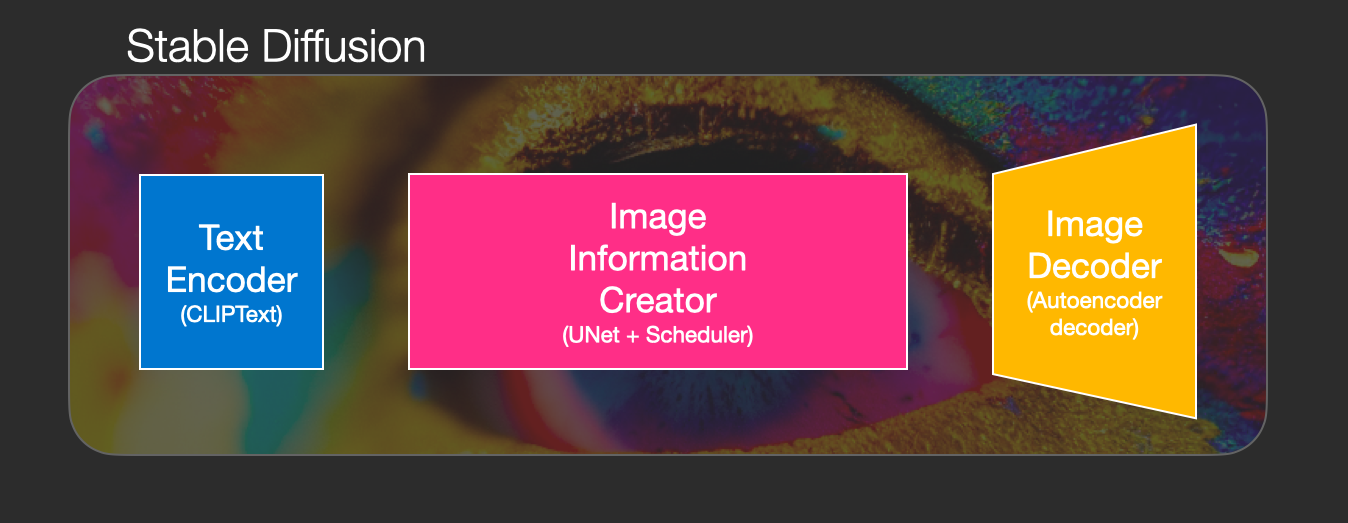
\includegraphics[width=0.90\textwidth]{images/ldm_components.png}
    \captionof{figure}{Ba thành phần của Stable Diffusion: (1) \textbf{Text Encoder} (CLIPText) chuyển prompt thành embedding, (2) \textbf{Image Information Creator} (U-Net + Scheduler) khử nhiễu lặp lại trong latent space, (3) \textbf{Image Decoder} (Autoencoder) chuyển latent thành ảnh pixel.}
    \label{fig:ldm_components}
\end{center}

\subsubsection{Thành phần 1: VAE --- Cánh cổng giữa Pixel và Latent}

\textbf{Variational Autoencoder (VAE)} là bộ phận mã hóa và giải mã không gian. Nó được huấn luyện \textit{trước} và \textit{độc lập} với phần diffusion.

\begin{center}
    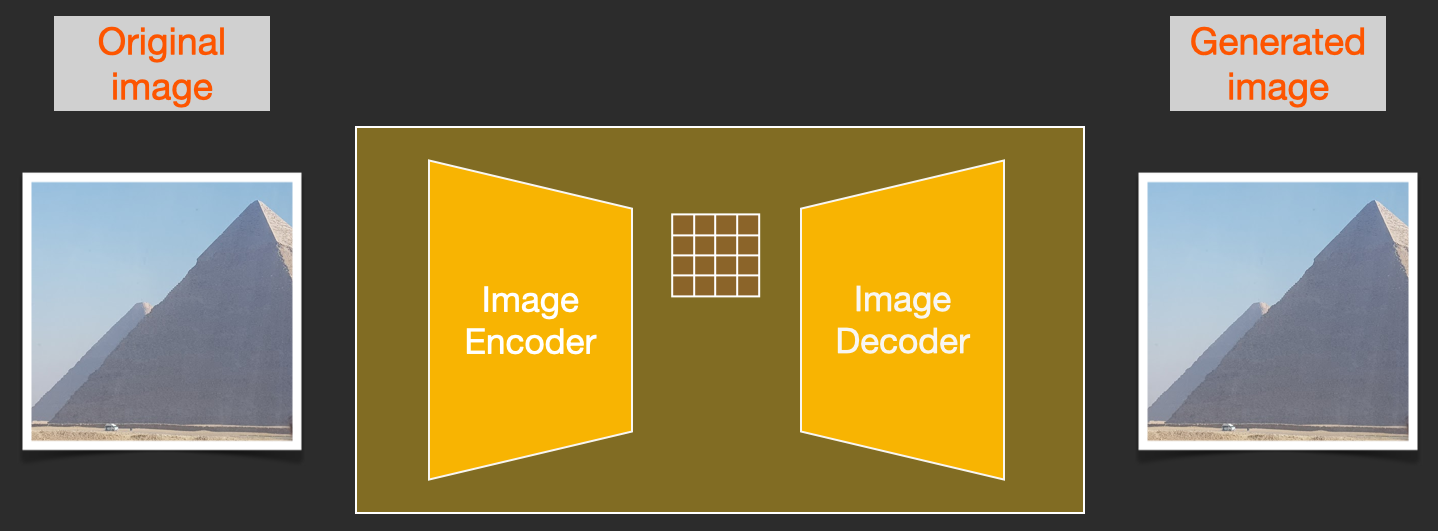
\includegraphics[width=0.88\textwidth]{images/ldm_vae.png}
    \captionof{figure}{VAE của Stable Diffusion: Image Encoder nén ảnh gốc $512\times512\times3$ thành latent $64\times64\times4$ (lưới nhỏ ở giữa), Image Decoder tái tạo ảnh từ latent. Encoder chỉ dùng khi training; trong inference chỉ cần Decoder.}
    \label{fig:ldm_vae}
\end{center}

\begin{itemize}
    \item \textbf{Encoder} $\mathcal{E}$: nhận ảnh $\mathbf{x} \in \mathbb{R}^{512 \times 512 \times 3}$, xuất ra latent $\mathbf{z} = \mathcal{E}(\mathbf{x}) \in \mathbb{R}^{64 \times 64 \times 4}$. Mỗi ``pixel'' trong latent tương ứng với một vùng $8 \times 8$ pixel gốc và mã hóa thông tin ngữ nghĩa của vùng đó.
    \item \textbf{Decoder} $\mathcal{D}$: nhận latent $\mathbf{z}$, tái tạo ảnh $\hat{\mathbf{x}} = \mathcal{D}(\mathbf{z}) \approx \mathbf{x}$. Trong inference, đây là bước cuối cùng sau khi denoising xong.
\end{itemize}

VAE được huấn luyện để nén ảnh nhưng vẫn giữ lại thông tin đủ để tái tạo chân thực. Trong inference, \textit{chỉ cần Decoder} --- Encoder không được sử dụng (không có ảnh gốc để encode).

\subsubsection{Thành phần 2: CLIP Text Encoder --- Dịch Chữ thành Số}

Để mô hình ``hiểu'' prompt văn bản, Stable Diffusion dùng \textbf{CLIP} (Contrastive Language-Image Pretraining) --- một mô hình được OpenAI huấn luyện trên 400 triệu cặp ảnh-văn bản từ internet.

CLIP học một không gian embedding chung cho cả ảnh và văn bản: những ảnh và caption mô tả cùng một thứ sẽ có embedding gần nhau. Kết quả là CLIP text encoder ``hiểu'' ngữ nghĩa sâu hơn một language model thông thường --- nó biết ``a fluffy golden retriever'' và ``a dog with curly golden fur'' đều gần nhau trong embedding space.

\textbf{Quá trình xử lý text}: Prompt được tokenize thành tối đa 77 token, mỗi token được embed thành vector 768 chiều. Kết quả là tensor $\mathbf{c} \in \mathbb{R}^{77 \times 768}$ --- ``bản tóm tắt ngữ nghĩa'' của toàn bộ prompt.

\subsubsection{Thành phần 3: U-Net trong Latent Space --- Trái tim của quá trình sinh ảnh}

U-Net trong Stable Diffusion nhận \textit{ba} đầu vào đồng thời và dự đoán nhiễu cần loại bỏ:

\begin{center}
    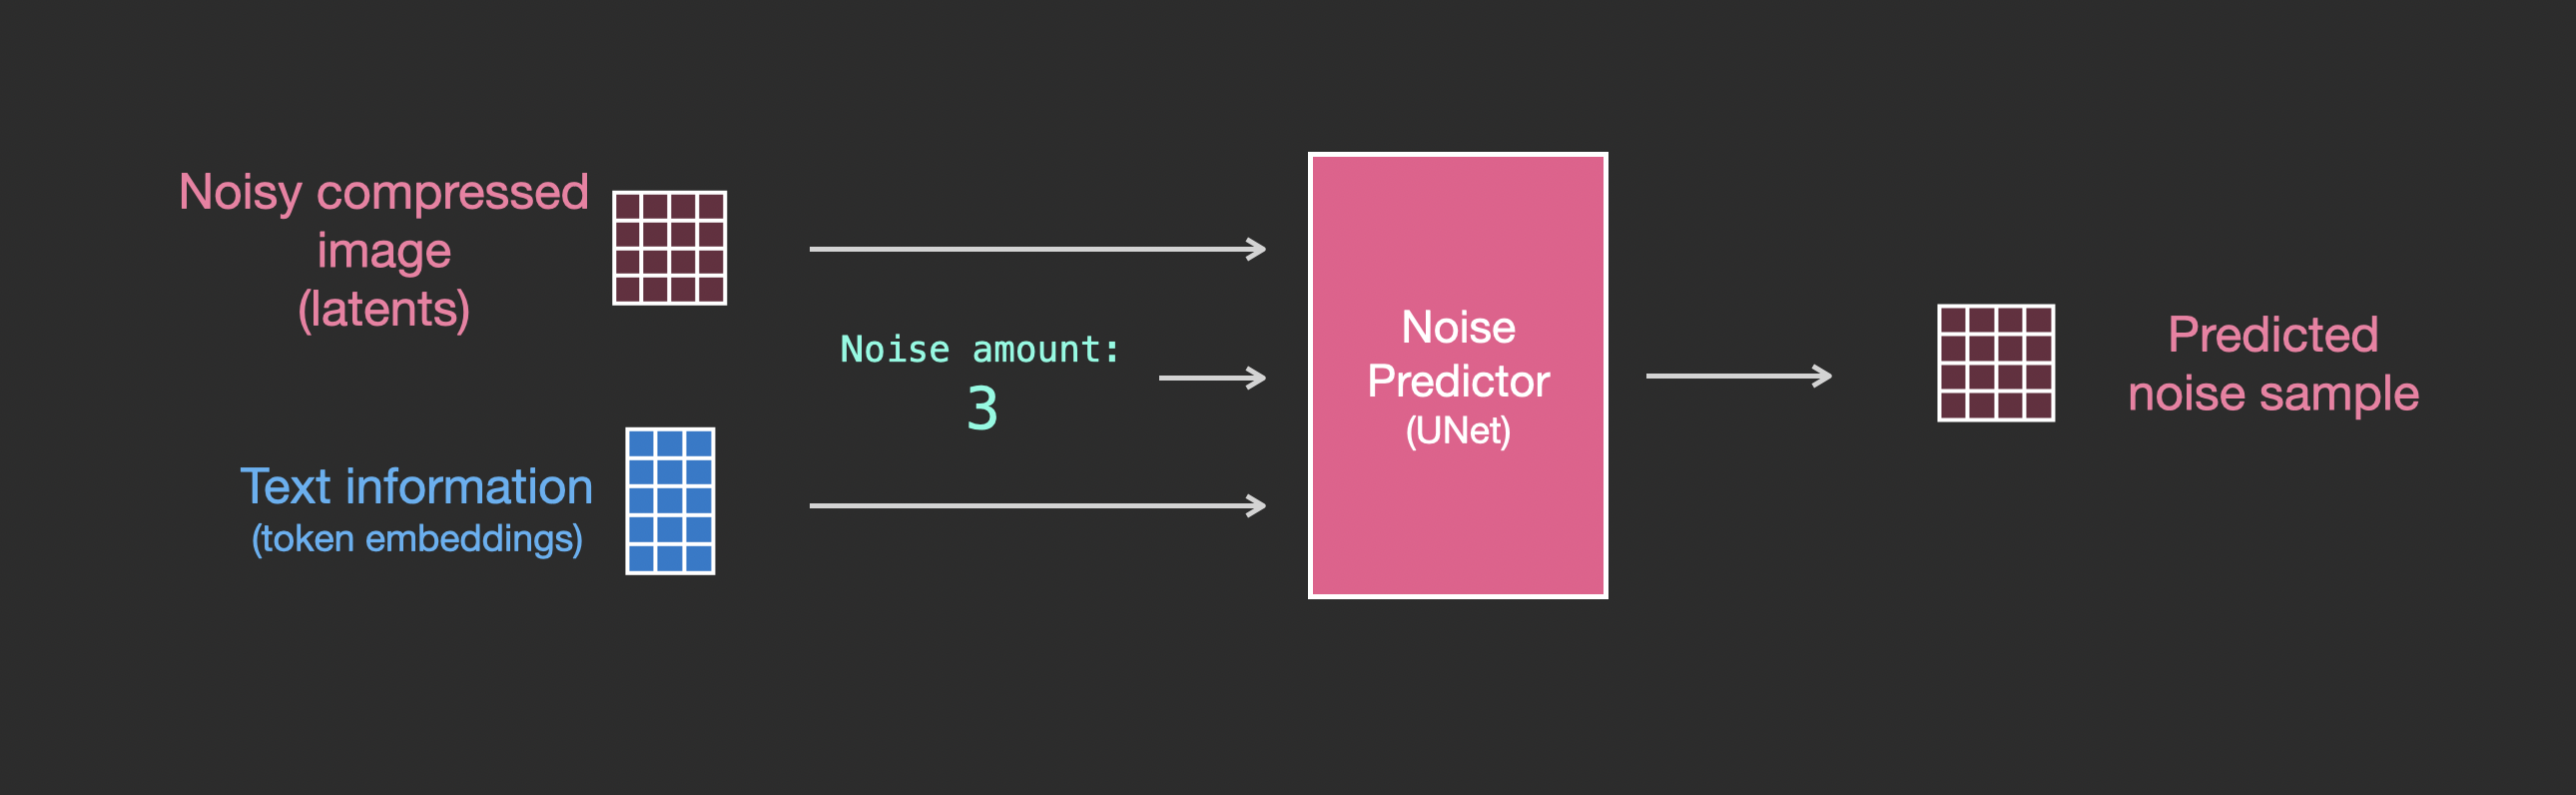
\includegraphics[width=0.95\textwidth]{images/ldm_unet_text.png}
    \captionof{figure}{U-Net (Noise Predictor) nhận ba đầu vào: latent nhiễu ($64\times64\times4$), bước thời gian (noise amount), và text token embeddings ($77\times768$). Xuất ra predicted noise sample cùng kích thước với latent đầu vào.}
    \label{fig:ldm_unet_inputs}
\end{center}

\begin{enumerate}
    \item \textbf{Noisy latent} $\mathbf{z}_t \in \mathbb{R}^{64 \times 64 \times 4}$: latent ở bước $t$ (đang chứa nhiễu).
    \item \textbf{Timestep} $t$: bước thời gian hiện tại (encoded bằng sinusoidal embedding).
    \item \textbf{Text embedding} $\mathbf{c} \in \mathbb{R}^{77 \times 768}$: từ CLIP text encoder.
\end{enumerate}

\textbf{Cross-Attention --- Cơ chế kết nối text và ảnh.}
Text embedding $\mathbf{c}$ được tích hợp vào U-Net qua các lớp \textbf{cross-attention} xen kẽ giữa các ResNet block. Tại mỗi lớp attention:

\[
    \text{Attention}(\mathbf{Q}, \mathbf{K}, \mathbf{V}) = \text{softmax}\!\left(\frac{\mathbf{Q}\mathbf{K}^\top}{\sqrt{d}}\right)\mathbf{V}
\]

\begin{itemize}
    \item $\mathbf{Q}$ (Query) đến từ \textit{latent features} --- ``ảnh đang hỏi: tôi cần thông tin gì từ prompt?''
    \item $\mathbf{K}, \mathbf{V}$ (Key, Value) đến từ \textit{text embedding} $\mathbf{c}$ --- ``prompt trả lời: đây là thông tin tôi có.''
\end{itemize}

Nhờ đó, ở mỗi vị trí không gian trong latent, U-Net ``hỏi'' text embedding xem token nào liên quan nhất đến vùng đó và điều chỉnh denoising cho phù hợp. Ví dụ: khi xử lý vùng latent tương ứng với bầu trời, attention cao vào token ``blue sky''; khi xử lý vùng tiền cảnh, attention cao vào token mô tả vật thể chính.

\begin{center}
    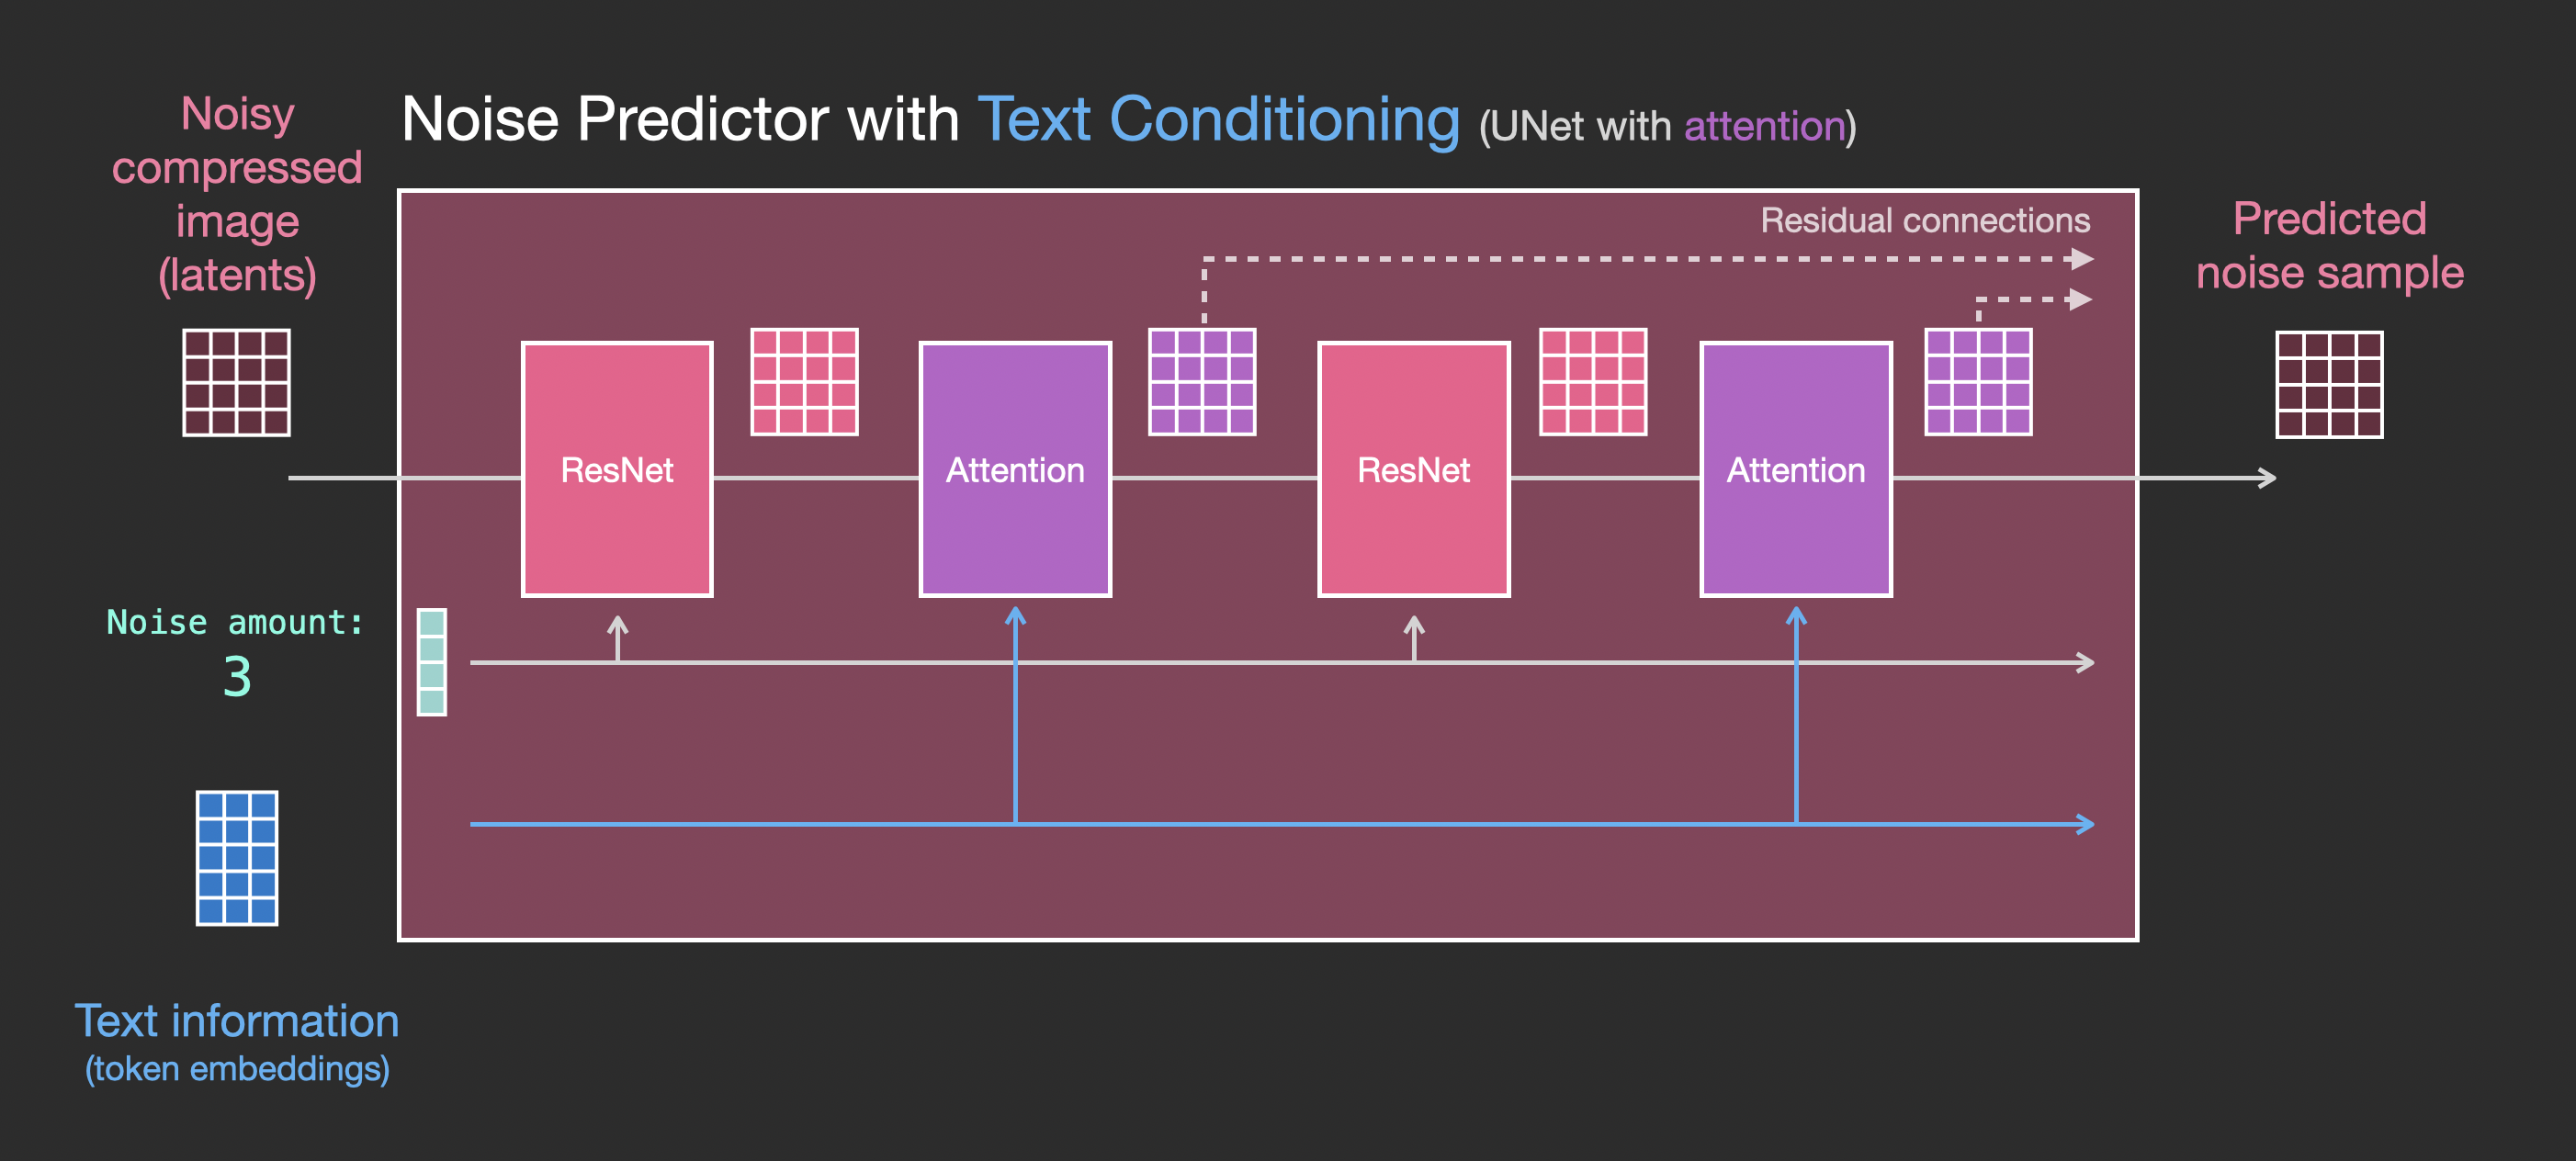
\includegraphics[width=0.98\textwidth]{images/ldm_unet_steps.png}
    \captionof{figure}{Kiến trúc U-Net với text conditioning: xen kẽ ResNet blocks (xử lý không gian) và Attention blocks (kết hợp text qua cross-attention). Text information được inject ở mỗi Attention block, đảm bảo hướng dẫn sinh ảnh xuyên suốt từ encoder đến decoder.}
    \label{fig:ldm_unet_text}
\end{center}

\subsubsection{Pipeline hoàn chỉnh: Từ Văn bản đến Ảnh}

Khi nhận prompt \textit{``a majestic lion at sunset, oil painting style''}:

\begin{center}
    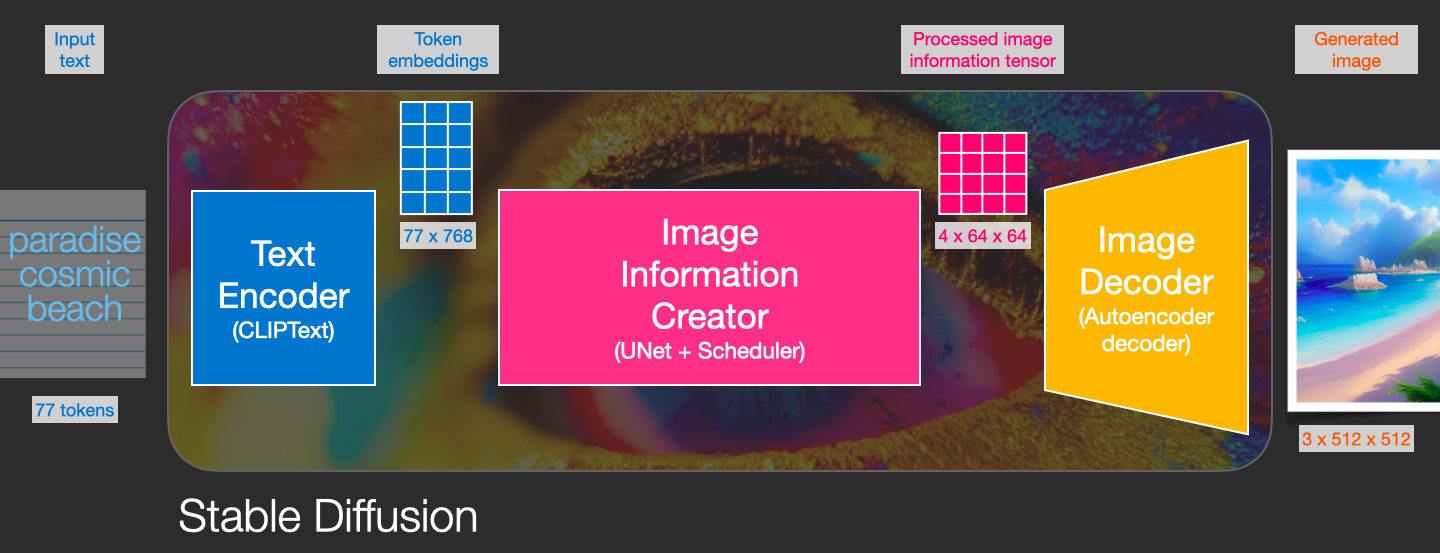
\includegraphics[width=0.95\textwidth]{images/ldm_tensors.png}
    \captionof{figure}{Pipeline đầy đủ với kích thước tensor cụ thể: text prompt → 77 token × 768 chiều; latent nhiễu ban đầu $4\times64\times64$; sau 50 bước denoising với U-Net → latent sạch $4\times64\times64$; VAE decoder → ảnh $512\times512\times3$.}
    \label{fig:ldm_full_pipeline}
\end{center}

\begin{enumerate}
    \item \textbf{Encode text}: CLIP text encoder chuyển prompt thành $\mathbf{c} \in \mathbb{R}^{77 \times 768}$.
    \item \textbf{Khởi tạo}: Lấy mẫu latent nhiễu ngẫu nhiên $\mathbf{z}_T \sim \mathcal{N}(\mathbf{0}, \mathbf{I})$, kích thước $4 \times 64 \times 64$.
    \item \textbf{Denoising loop} ($T = 50$--$100$ bước với DDIM scheduler):
    \begin{itemize}
        \item U-Net dự đoán nhiễu: $\hat{\boldsymbol{\epsilon}} = \boldsymbol{\epsilon}_\theta(\mathbf{z}_t, t, \mathbf{c})$
        \item Áp dụng CFG: kết hợp dự đoán có/không prompt với guidance scale $w$
        \item Tính $\mathbf{z}_{t-1}$ bằng cách trừ nhiễu dự đoán
    \end{itemize}
    \item \textbf{Decode}: VAE decoder chuyển latent sạch $\mathbf{z}_0 \in \mathbb{R}^{4 \times 64 \times 64}$ thành ảnh $\hat{\mathbf{x}} \in \mathbb{R}^{512 \times 512 \times 3}$.
\end{enumerate}

\begin{center}
    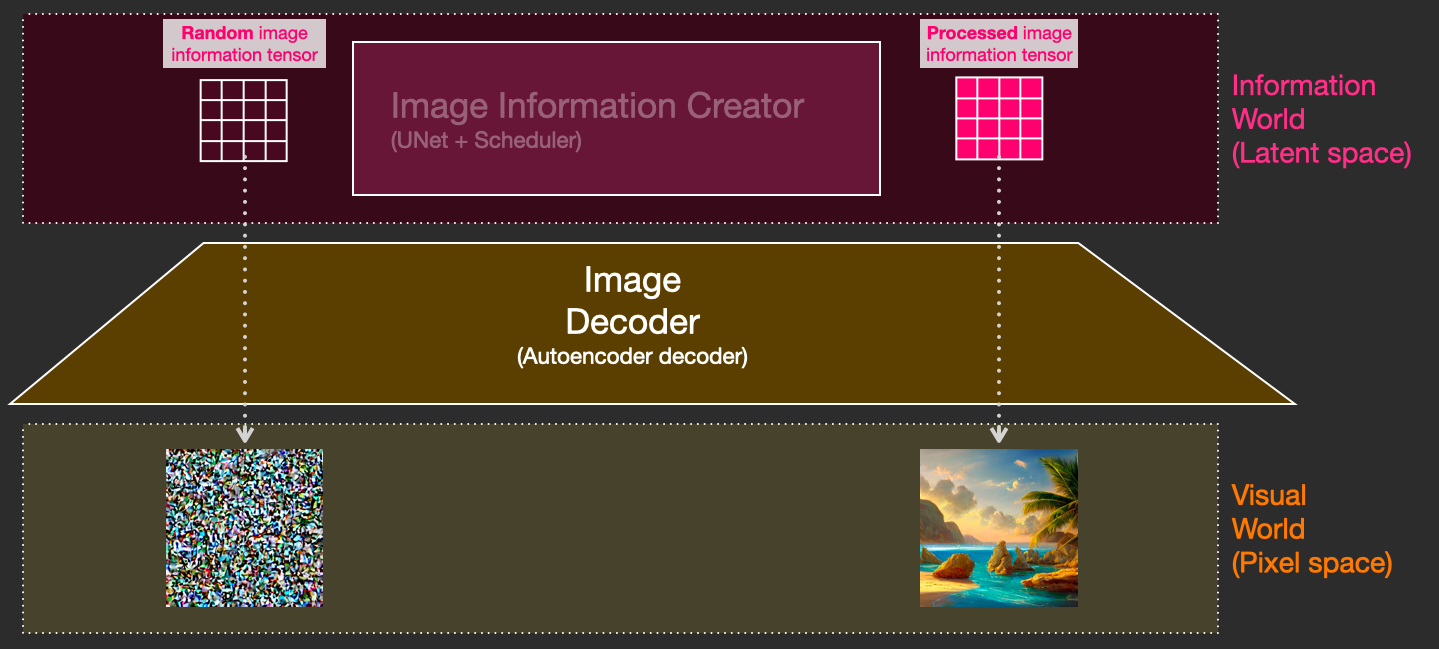
\includegraphics[width=0.90\textwidth]{images/ldm_latent_vs_pixel.png}
    \captionof{figure}{Hai thế giới trong Stable Diffusion: \textbf{Information World} (latent space) nơi U-Net làm việc với tensor nhỏ $4\times64\times64$, và \textbf{Visual World} (pixel space) nơi con người nhìn thấy ảnh $512\times512$. VAE Decoder là cầu nối duy nhất từ latent xuống pixel.}
    \label{fig:ldm_two_worlds}
\end{center}

\textbf{Stable Diffusion} (Rombach et al., 2022) là phiên bản LDM được huấn luyện trên \textbf{LAION-5B} --- bộ dữ liệu 5.8 tỷ cặp ảnh-văn bản thu thập từ internet. Điểm đặc biệt: được phát hành \textbf{mã nguồn mở} với trọng số công khai, tạo ra cả một hệ sinh thái cộng đồng khổng lồ (Civitai, HuggingFace, ComfyUI...). Các phiên bản tiếp theo như \textbf{SDXL} (2023) nâng độ phân giải lên $1024 \times 1024$ và cải thiện chất lượng đáng kể; \textbf{SD 3.0} (2024) dùng kiến trúc Diffusion Transformer thay thế U-Net.

\begin{mdframed}[style=infobox]
\textbf{Tại sao Stable Diffusion nhanh hơn DALL-E hay Midjourney thế hệ đầu?}

DALL-E v1 (OpenAI, 2021) dùng VQ-VAE + Transformer trên token rời rạc --- chậm và giới hạn độ phân giải. Midjourney v1 dùng pixel-space diffusion. Stable Diffusion thực hiện tất cả denoising trong latent $64\times64$ thay vì pixel $512\times512$ --- tức là mỗi bước U-Net nhanh hơn \textbf{48 lần}. Với 50 bước DDIM thay vì 1000 bước DDPM, tổng tốc độ tăng gấp hàng nghìn lần so với DDPM pixel-space gốc. Đây là lý do Stable Diffusion có thể chạy trên laptop consumer GPU 8GB VRAM.
\end{mdframed}
\subsection{Kỹ thuật Điều khiển Quá trình Sinh ảnh}
\label{subsec:diffusion_control_techniques}

Sức mạnh thực sự của các mô hình khuếch tán không chỉ nằm ở khả năng tạo ra các ảnh ngẫu nhiên chất lượng cao, mà còn ở khả năng kiểm soát và tùy chỉnh quá trình sinh một cách tinh vi. Nhiều kỹ thuật gần đây cho phép chúng ta điều khiển nội dung, bố cục, phong cách, và thậm chí là các đối tượng cụ thể trong ảnh.

\begin{description}
	\item[Textual Inversion:] \cite{Gal2022_textual} 
	\begin{itemize}
		\item \textbf{Mục tiêu:} Cho phép mô hình học một khái niệm thị giác mới từ chỉ một vài (3-5) bức ảnh, mà không cần huấn luyện lại toàn bộ mô hình.
		\item \textbf{Cơ chế:} 
		\begin{enumerate}
			\item Giữ "đóng băng" toàn bộ mô hình diffusion và text encoder.
			\item Tối ưu hóa một embedding vector mới trong từ vựng của text encoder, ví dụ `S*`.
			\item Vector `S*` có thể được dùng trong prompt như một từ khóa: \textit{"a photo of S* in the style of Van Gogh"}.
		\end{enumerate}
		\item \textbf{Ưu điểm:} Nhanh, tiết kiệm tài nguyên, dễ tích hợp vào pipeline hiện có.
		\item \textbf{Hạn chế:} Khả năng tạo ra các chi tiết phức tạp hoặc phong cách đặc trưng đôi khi kém hơn các phương pháp fine-tune.
	\end{itemize}
	
	\item[DreamBooth:] \cite{Ruiz2023_dreambooth}
	\begin{itemize}
		\item \textbf{Mục tiêu:} Cá nhân hóa mô hình diffusion để sinh ra các đối tượng hoặc phong cách cụ thể với độ chính xác cao.
		\item \textbf{Cơ chế:} 
		\begin{enumerate}
			\item Thay vì chỉ học một embedding, DreamBooth tinh chỉnh một phần nhỏ của toàn bộ U-Net.
			\item Sử dụng một định danh lớp hiếm (rare class token), ví dụ `sks`, để tránh quên các khái niệm gốc: \textit{"a photo of a sks dog"}.
			\item Kết hợp dữ liệu ảnh mới của đối tượng với prompt để mô hình học cả nội dung và phong cách đặc trưng.
		\end{enumerate}
		\item \textbf{Ưu điểm:} Tạo ảnh cá nhân hóa rất chính xác, duy trì các chi tiết đặc trưng của đối tượng.
		\item \textbf{Hạn chế:} Yêu cầu nhiều tài nguyên hơn so với Textual Inversion và quá trình fine-tune cần cẩn trọng để tránh "overfitting".
	\end{itemize}
	
	\item[ControlNet:] \cite{Zhang2023_controlnet}
	\begin{itemize}
		\item \textbf{Mục tiêu:} Tăng khả năng điều khiển chi tiết quá trình sinh ảnh bằng các điều kiện không gian như đường viền (edges), tư thế (pose), độ sâu (depth map) hoặc phác thảo (scribbles).
		\item \textbf{Kiến trúc:} 
		\begin{enumerate}
			\item Đóng băng toàn bộ mô hình diffusion lớn đã được huấn luyện trước (như Stable Diffusion).
			\item Tạo một bản sao của các khối mã hóa trong mô hình gốc và huấn luyện bản sao này (gọi là "ControlNet") để nhận thêm đầu vào điều kiện.
			\item Output từ ControlNet được cộng vào output của các lớp tương ứng trong mô hình diffusion gốc, "hướng dẫn" quá trình khử nhiễu theo cấu trúc mong muốn.
		\end{enumerate}
		\item \textbf{Quá trình hoạt động:} 
		\begin{itemize}
			\item Nhập ảnh điều kiện (ví dụ: skeleton pose, edge map) vào ControlNet.
			\item ControlNet điều chỉnh các đặc trưng trong quá trình diffusion, đảm bảo ảnh sinh ra tuân theo bố cục/chi tiết của điều kiện.
		\end{itemize}
		\item \textbf{Ưu điểm:} 
		\begin{itemize}
			\item Cho phép kiểm soát chính xác bố cục, tư thế, và các chi tiết hình học.
			\item Dễ kết hợp với các kỹ thuật điều kiện khác như Text-to-Image hoặc DreamBooth.
		\end{itemize}
		\item \textbf{Hạn chế:} Yêu cầu ảnh điều kiện phù hợp và đôi khi tăng chi phí tính toán.
	\end{itemize}
\end{description}

\begin{center}
	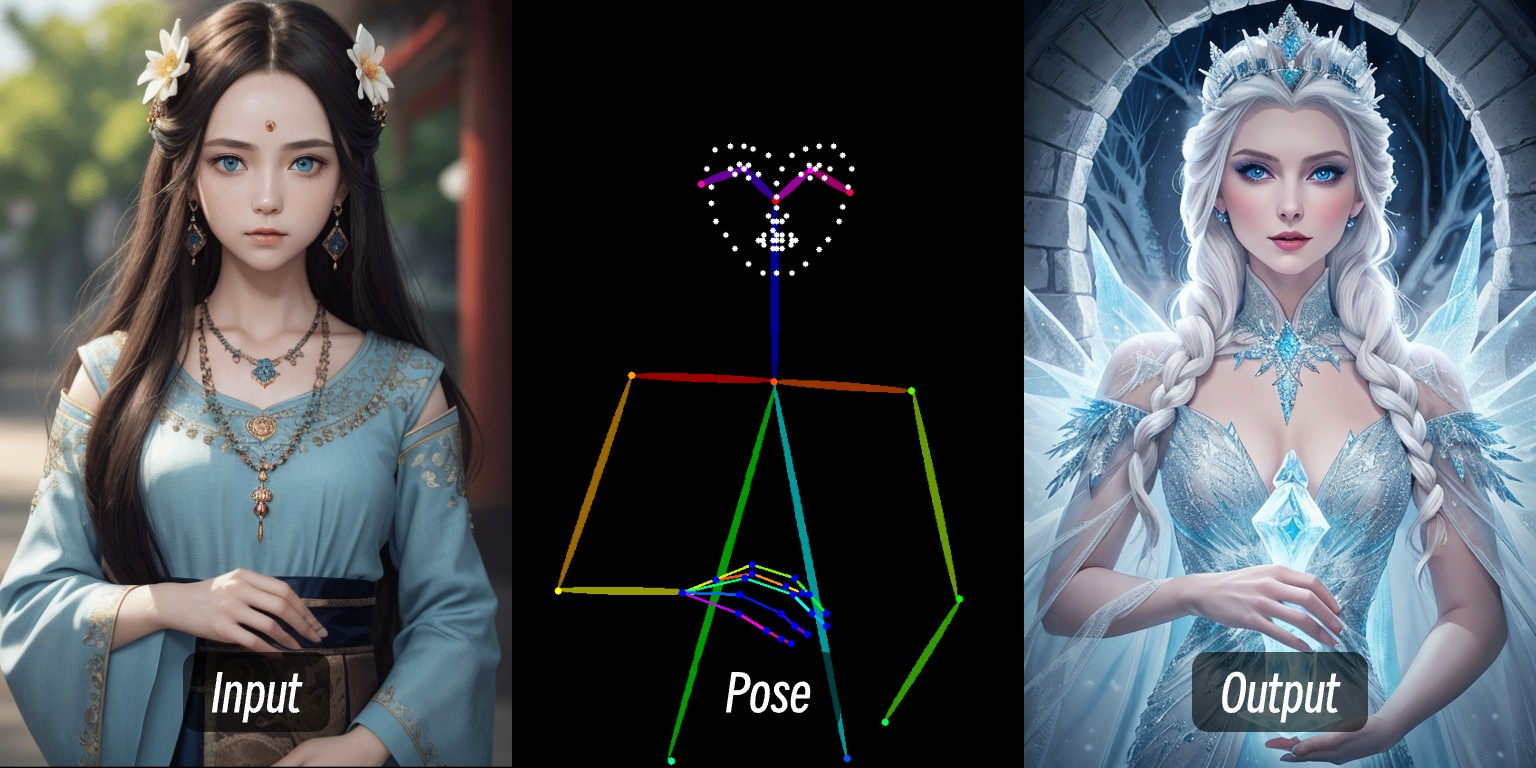
\includegraphics[width=1.0\textwidth]{images/controlnet_pose_example.jpg}
	\captionof{figure}{Ví dụ về ControlNet: bằng cách cung cấp một ảnh tư thế (pose) làm điều kiện, ControlNet hướng dẫn mô hình diffusion (Stable Diffusion) tạo ra nhân vật với tư thế chính xác.}
	\label{fig:controlnet_example}
\end{center}

\subsection{Kết luận: Một Kỷ nguyên Mới của Sáng tạo Thị giác}
\label{subsec:diffusion_conclusion}
Các mô hình khuếch tán đã thay đổi cuộc chơi trong lĩnh vực AI sáng tạo. Chúng không chỉ vượt qua GANs về chất lượng và sự đa dạng của ảnh sinh ra, mà còn cung cấp một nền tảng ổn định và cực kỳ linh hoạt để điều khiển quá trình sáng tạo.

Từ nền tảng lý thuyết của DDPM, sự tối ưu hóa hiệu quả của Latent Diffusion, đến khả năng kiểm soát tinh vi của ControlNet, DreamBooth, và Textual Inversion, các mô hình khuếch tán đã dân chủ hóa khả năng sáng tạo nghệ thuật, biến những ý tưởng trong văn bản thành những tác phẩm thị giác chi tiết. Chúng là công nghệ cốt lõi đằng sau cuộc cách mạng text-to-image và đang nhanh chóng được mở rộng sang các lĩnh vực video, 3D, và âm thanh, hứa hẹn một tương lai nơi ranh giới giữa trí tưởng tượng của con người và khả năng tổng hợp của máy móc ngày càng bị xóa nhòa.

\section*{Tài liệu tham khảo}
\begin{itemize}
	\item[1] Ho, J., Jain, A., \& Abbeel, P. (2020). Denoising diffusion probabilistic models. In \textit{Advances in Neural Information Processing Systems (NeurIPS)}. (Paper gốc giới thiệu DDPM).
	\item[2] Rombach, R., Blattmann, A., Lorenz, D., Esser, P., \& Ommer, B. (2022). High-resolution image synthesis with latent diffusion models. In \textit{Proceedings of the IEEE/CVF Conference on Computer Vision and Pattern Recognition (CVPR)}. (Paper gốc giới thiệu Latent Diffusion Models, nền tảng của Stable Diffusion).
	\item[3] Zhang, L., \& Agrawala, M. (2023). Adding conditional control to text-to-image diffusion models. In \textit{Proceedings of the IEEE/CVF International Conference on Computer Vision (ICCV)}. (Paper gốc giới thiệu ControlNet).
	\item[4] Gal, R., Alaluf, Y., Atzmon, Y., Patashnik, O., Bermano, A. H., \& Cohen-Or, D. (2022). An image is worth one word: Personalizing text-to-image generation using textual inversion. In \textit{ECCV Workshops}. (Paper gốc giới thiệu Textual Inversion).
	\item[5] Ruiz, N., Li, Y., Jampani, V., Pritch, Y., Rubinstein, M., \& Aberman, K. (2023). Dreambooth: Fine-tuning text-to-image diffusion models for subject-driven generation. In \textit{Proceedings of the IEEE/CVF Conference on Computer Vision and Pattern Recognition (CVPR)}. (Paper gốc giới thiệu DreamBooth).
	\item[6] Dhariwal, P., \& Nichol, A. (2021). Diffusion models beat GANs on image synthesis. In \textit{Advances in Neural Information Processing Systems (NeurIPS)}. (Paper giới thiệu Classifier Guidance).
	\item[7] Ho, J., \& Salimans, T. (2022). Classifier-free diffusion guidance. In \textit{NeurIPS Workshop on Deep Generative Models}. (Paper giới thiệu Classifier-Free Guidance - CFG).
	\item[8] Sohl-Dickstein, J., Weiss, E., Maheswaranathan, N., \& Ganguli, S. (2015). Deep unsupervised learning using nonequilibrium thermodynamics. In \textit{International Conference on Machine Learning (ICML)}. (Một trong những công trình lý thuyết sơ khai đặt nền móng cho các mô hình khuếch tán).
\end{itemize}